\documentclass[10pt,aspectratio=169]{beamer}
% \documentclass[10pt,aspectratio=169,handout]{beamer}

% silence some Metropolis warnings
\usepackage{silence}
\WarningFilter{beamerthememetropolis}{You need to compile with XeLaTeX or LuaLaTeX}
\WarningFilter{latexfont}{Font shape}
\WarningFilter{latexfont}{Some font}

% define custom colors
\definecolor{dark gray}{HTML}{444444}
\definecolor{light gray}{HTML}{777777}
\definecolor{dark red}{HTML}{BB0000}
\definecolor{dark green}{HTML}{00BB00}

% configure metropolis
\usetheme[numbering=fraction]{metropolis}
\setbeamercolor{background canvas}{bg=white}
\setbeamercolor{frametitle}{bg=dark gray}
\setbeamercolor{alerted text}{fg=dark red}
\setbeamercolor{item projected}{bg=dark red}
\setbeamercolor{local structure}{fg=dark red}
\setbeamersize{text margin left=0.5cm,text margin right=0.5cm}
\setbeamercovered{transparent=10}

% use thicker lines
\makeatletter
\setlength{\metropolis@titleseparator@linewidth}{1pt}
\setlength{\metropolis@progressonsectionpage@linewidth}{1pt}
\makeatother

% custom bullet points
\setbeamertemplate{itemize item}{\color{dark red}$\blacktriangleright$}
\setbeamertemplate{itemize subitem}{\color{dark red}$\blacktriangleright$}
\setbeamertemplate{itemize subsubitem}{\color{dark red}$\blacktriangleright$}
\newcommand{\custombullet}{{\color{dark red}$\blacktriangleright$}\hspace{0.5em}}

% use classic font for math
\usefonttheme[onlymath]{serif}

% imports
\usepackage[english]{babel}
\usepackage[utf8]{inputenc}
\usepackage{amsthm}
\usepackage{amssymb}
\usepackage{amsmath}
\usepackage{amsfonts}
\usepackage{mathtools}
\usepackage{mathabx}
\usepackage{stmaryrd}
\usepackage{graphicx}
\usepackage{hyperref}
\usepackage{xfrac}
\usepackage{appendixnumberbeamer}

% check and x marks
\usepackage{pifont}
\newcommand{\cmark}{{\color{dark green}\ding{51}}\hspace{0.3em}}
\newcommand{\xmark}{{\color{dark red}\ding{55}}\hspace{0.5em}}

% diagrams
\usepackage{tikz}
\usetikzlibrary{decorations.pathreplacing}

% references
\usepackage[natbibapa]{apacite}
\bibliographystyle{apacite}
\renewcommand{\bibsection}{}

% use ampersands instead of "and" for text citations
\AtBeginDocument{\renewcommand{\BBAB}{\&}}

% possessive cites
\makeatletter
\patchcmd{\NAT@test}{\else \NAT@nm}{\else \NAT@nmfmt{\NAT@nm}}{}{}
\DeclareRobustCommand\citepos
  {\begingroup
   \let\NAT@nmfmt\NAT@posfmt
   \NAT@swafalse\let\NAT@ctype\z@\NAT@partrue
   \@ifstar{\NAT@fulltrue\NAT@citetp}{\NAT@fullfalse\NAT@citetp}}
\let\NAT@orig@nmfmt\NAT@nmfmt
\def\NAT@posfmt#1{\NAT@orig@nmfmt{#1's}}
\makeatother

% spaced-out lists
\newenvironment{wideitemize}{\itemize\addtolength{\itemsep}{10pt}}{\enditemize}
\newenvironment{wideenumerate}{\enumerate\addtolength{\itemsep}{10pt}}{\endenumerate}

% replace footnotes with buttons
\usepackage[absolute,overlay]{textpos}
\newcounter{beamerpausessave}
\newcommand{\always}[1]{
    \setcounter{beamerpausessave}{\value{beamerpauses}}
    \setcounter{beamerpauses}{0}
    \pause
    #1 
    \setcounter{beamerpauses}{\value{beamerpausessave}}
    \addtocounter{beamerpauses}{-1}
    \pause
}
\newcommand{\buttons}[1]{\always{
    \begin{textblock*}{\paperwidth}(0.015\textwidth, 1.022\textheight)
        \scriptsize
        #1
    \end{textblock*}
}}
\newcommand{\appendixbuttons}[1]{\always{
    \begin{textblock*}{\paperwidth}(0.015\textwidth, 1.043\textheight)
        \scriptsize
        #1
    \end{textblock*}
}}
\newcommand{\goto}[2]{\hyperlink{#1}{{\color{dark red}$\smalltriangleright$} #2}\hspace{0.5em}}
\newcommand{\goback}[2]{\hyperlink{#1}{{\color{dark red}$\smalltriangleleft$} #2}\hspace{0.5em}}

% custom appendix
\renewcommand{\appendixname}{\texorpdfstring{\translate{Appendix}}{Appendix}}

% change color of cites and URLs
\let\oldcite\cite
\let\oldcitet\citet
\let\oldcitep\citep
\let\oldcitepos\citepos
\let\oldcitetalias\citetalias
\let\oldcitepalias\citepalias
\let\oldurl\url
\def\cite#1#{\citeaux{#1}}
\def\citet#1#{\citetaux{#1}}
\def\citep#1#{\citepaux{#1}}
\def\citepos#1#{\citeposaux{#1}}
\def\citetalias#1#{\citetaliasaux{#1}}
\def\citepalias#1#{\citepaliasaux{#1}}
\def\url#1#{\urlaux{#1}}
\newcommand*\citeaux[2]{{\color{light gray}\oldcite#1{#2}}}
\newcommand*\citetaux[2]{{\color{light gray}\oldcitet#1{#2}}}
\newcommand*\citepaux[2]{{\color{light gray}\oldcitep#1{#2}}}
\newcommand*\urlaux[2]{{\color{light gray}\oldurl#1{#2}}}
\newcommand*\citeposaux[2]{{\color{light gray}\oldcitepos#1{#2}}}
\newcommand*\citetaliasaux[2]{{\color{light gray}\oldcitetalias#1{#2}}}
\newcommand*\citepaliasaux[2]{{\color{light gray}\oldcitepalias#1{#2}}}

% custom math commands
\DeclareMathOperator*{\argmax}{argmax}
\DeclareMathOperator*{\argmin}{argmin}
\renewcommand{\Pr}{\mathbb{P}}
\newcommand{\E}{\mathbb{E}}
\newcommand{\Var}{\mathbb{V}}
\newcommand{\Cov}{\mathbb{C}}
\newcommand{\overbar}[1]{\mkern 1.5mu\overline{\mkern-1.5mu#1\mkern-1.5mu}\mkern 1.5mu}

% tables
\usepackage{booktabs}
\usepackage{colortbl}
\usepackage{multirow}
\usepackage{makecell}
\arrayrulecolor{dark red}

% custom date
\usepackage{datetime}
\newdateformat{monthyeardate}{\monthname[\THEMONTH] \THEYEAR}

% fix pauses with graphics
\usepackage{fixpauseincludegraphics}


\usepackage{tabularx}
\usepackage{dcolumn}
\usepackage{ragged2e}
\usepackage{multirow,multicol,dcolumn}




\begin{document}
\title{Pass Through}
\author{Chris Conlon}
\institute{Leuven Lectures}
\date{\today}

\frame{\titlepage}


\begin{frame}{Pass-Through: What is it?}
Lots of cases in economics where we want to know how prices respond to changes in costs:

\begin{itemize}
    \item Response to cost shocks (oil shock, commodity prices)
    \item Response to tax changes (incidence/efficiency of taxes)
    \item Transmission of Exchange Rate Shocks
    \item Transmission of Monetary Policy
    \item Price effects of Mergers
    \item Double Marginalization
\end{itemize}
\end{frame}


\begin{frame}{Hot take}
Pass-through is the simplest thing in economics that nobody understands
\begin{itemize}
\item Often we are talking about different things
\begin{itemize}
\item IO: mostly $\rho = \frac{\partial p_j}{\partial mc_j}$ or the matrix $\frac{\partial \mathbf{p}}{\partial \mathbf{mc}}$
\item Macro/Trade: mostly $\frac{\partial \log p_j}{\partial \log mc_j}$
\end{itemize}
\item One thing we know for sure: constant marginal costs, perfect competition: \\
 $$p = mc \rightarrow \frac{\partial \mathbf{p}}{\partial \mathbf{mc}} = 1$$
 \item Everything else depends on:
\begin{itemize}
\item Curvature of demand
\item Nature of competition
\end{itemize}
\end{itemize}
\end{frame}

\begin{frame}{How bad is it?: International Trade Edition}
Theory of International Trade
\begin{itemize}
\item Most models assume CES and monopolistic competition
\item Implied PT in exchange rate shocks (zero if in local currency, 100\% if in foreign currency).
\end{itemize}

Empirical Results International Trade:
\begin{itemize}
\item Gopinath, Ithshoki Rigobon (2010): 25\% if priced in dollars; 95\% if not.
\item Goldberg Hellerstein (2013): around 25\% of exchange rate shocks show up in retail beer prices
\item Nakamura Zerom: around 30\% of commodity price shocks for coffee show up in retail prices.
\end{itemize}
\end{frame}

\begin{frame}{How bad is it?: Public Finance Edition}
\begin{itemize}
\item Tobacco: Harding et al. (2012) $\rho < 1$, while DeCicca et al. (2013) $\rho \approx 1$.
\item Gasoline: Taxes are fully passed through to consumers except when supply is inelastic or inventories were high (Marion and Muehlegger, 2011) but tax holidays $\rho << 1$ (Doyle Jr. and Samphantharak, 2008)
\item Sales Taxes: Poterba (1996) found that retail prices of clothing and personal care items $\rho \approx 1$ Besley and Rosen (1999) could not reject $\rho \approx 1$, but found evidence of $\rho >1$ half of the goods.
\item Alcohol:  Young and Bielinska-Kwapisz (2002) $\rho = (1.6,2.1)$ Kenkel (2005) $\rho=(1.47,2.1)$
\end{itemize}
Many studies of ``price elasticity'' for gasoline, cigarettes, tobacco, etc assume that $\rho=1$ and regress prices on tax changes to get elasticities: $\frac{\partial \log p}{\partial \log t} = \frac{\partial \log p}{\partial \log c}$ (!)
\end{frame}




\begin{frame}{Example Merger/UPP}
\footnotesize
Consider Bertrand FOC's for multi-product firm $j$:
\begin{align*}
\label{eq:best_response}
\rightarrow \nonumber p_j &=q_{j}(\mathbf{p}) \left[-\frac{\partial q_{j}}{\partial P_{j}}(\mathbf{p})\right]^{-1} + c_{j} + \sum_{k \in \mathcal{J}_{f} \setminus j} \left(p_{k}-c_{k}\right) \underbrace{\frac{\partial q_{k}}{\partial P_{j}}(\mathbf{p})\left[-\frac{\partial q_{j}}{\partial P_{j}}(\mathbf{p})\right]^{-1}}_{D_{jk}(\mathbf{p})}\\
p_j(p_{-j}) &= \underbrace{\frac{1}{1+1/\epsilon_{jj}(\mathbf{p})}}_{\text{Markup}} \left[ c_j + \sum_{k \in \mathcal{J}_{f} \setminus j}  (p_k-c_k) \cdot  D_{jk} (\mathbf{p}) \right].
\end{align*}
Mult-product pricing \alert{raises the opportunity cost} of selling $j$.
\end{frame}

\begin{frame}{Upward Pricing Pressure}
Agencies often calculate \alert{Upward Pricing Pressure} or UPP asks how merger \alert{changes} the opportunity cost:
\begin{align*}
\left[ c_j + \sum_{k \in \mathcal{J}_{f} \setminus j}  (p_k-c_k) \cdot  D_{jk} (\mathbf{p}) \right] \\
UPP_j = \Delta c_j + \sum_{k \in \mathcal{J}_{g}}  (p_k-c_k) \cdot  D_{jk} (\mathbf{p}) 
\end{align*}
\begin{itemize}
    \item How does the merger change the \alert{opportunity cost} for $j$?
    \item If the opportunity cost change is positive we say there is \alert{upward pricing pressure}
    \item But how much do we expect prices to rise?
\end{itemize}
\end{frame}


\begin{frame}{Jaffe Weyl (2013)}
\begin{itemize}
\item If we knew the \alert{pass-through rate} $\rho = \frac{\partial p_j}{\partial mc_j}$ we could convert $\Delta mc_j$ to $\Delta p_j$.
\item But we would have to know the \alert{matrix} $\frac{\partial \mathbf{p}}{\partial \mathbf{mc}}$, which is fine except it is $J \times J$ parameters (again).
\item We can place restrictions on this matrix (maybe diagonal, or maybe just  $\frac{\partial \mathbf{p}}{\partial \mathbf{mc}}=0.8$, etc.).
\item Miller, Ryan, Remer Sheu (2012/2016) did just that: simulate some mergers
\begin{itemize}
    \item Calculate UPP
    \item What if we had whole $\frac{\partial \mathbf{p}}{\partial \mathbf{mc}}$ matrix? just the diagonal? just the average diagonal?
\end{itemize}
\item some approximations are easier than others (depends on curvature of demand)
\end{itemize}
\end{frame}


\begin{frame}{Miller, Ryan, Remer Sheu}
\begin{columns}
\begin{column}{0.5\textwidth}
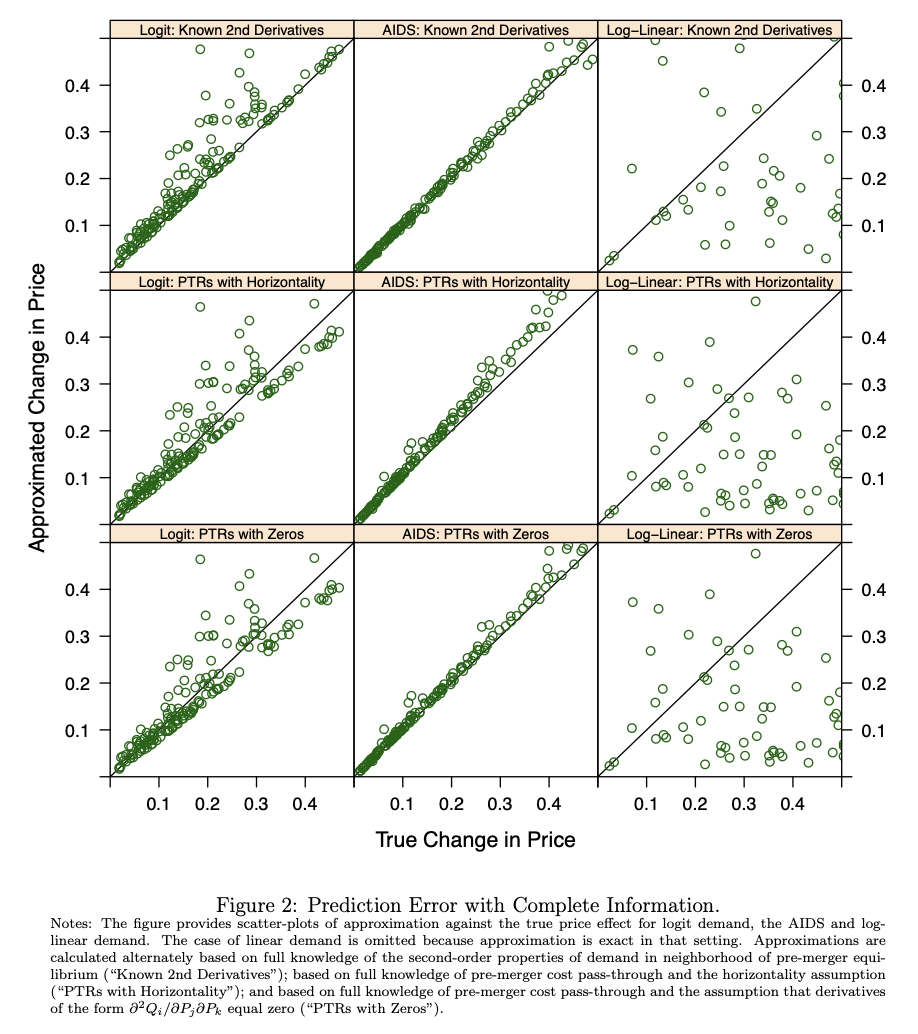
\includegraphics[width=\textwidth]{resources/mrss_complete}
\end{column}
\begin{column}{0.5\textwidth}
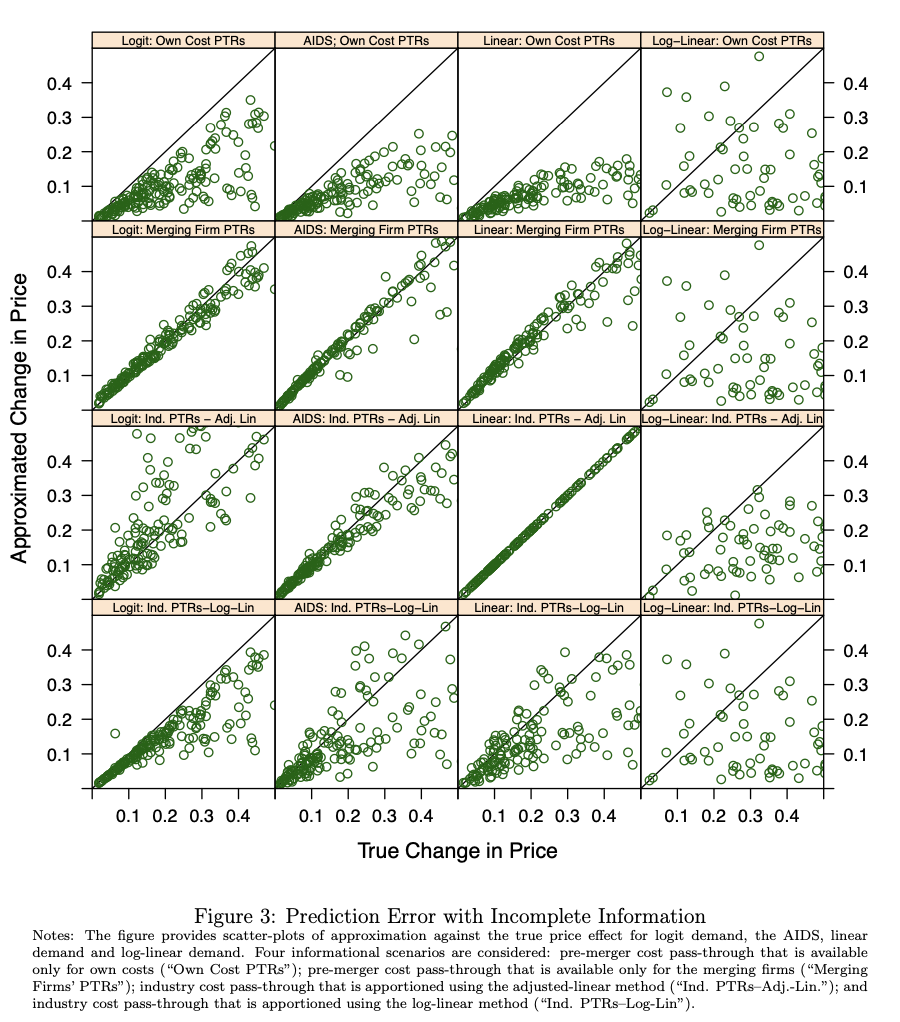
\includegraphics[width=\textwidth]{resources/mrss_incomplete}
\end{column}
\end{columns}
\end{frame}


\begin{frame}{Perfect Competition: Jenkin (1872), Alfred Marshall (1890)}
\begin{align*}
D(p) &= S(p-t)\\
\rho&= \frac{d p}{d t} = \frac{1}{1 + \frac{\varepsilon_d}{\varepsilon_s}}
\end{align*}

\begin{itemize}
\item Where $\varepsilon_d$ is \alert{demand elasticity} and $\varepsilon_s$ is \alert{supply elasticity} respectively.\\
\item $\rho \in [0,1]$ as long demand slopes down and supply slopes up!
\item Constant MC implies that $\varepsilon_s \rightarrow \infty$ and $\rho \rightarrow 1$
\item $I = \frac{\frac{d\, CS}{d\, t}}{\frac{d\, PS}{d\, t}} = \frac{\rho}{1-\rho}$ (higher pass-through more borne by consumers)
\end{itemize}
So far so good.
\end{frame}


\begin{frame}{Monopoly (Fabinger Weyl JPE)}
Start with $MR = MC$:
\begin{align*}
mr(q) = p(q) + p'(q) q &= mc(q) + t\\
m r^{\prime} \frac{d q}{d t} & =m c^{\prime} \frac{d q}{d t}+1 \Rightarrow \frac{d q}{d t}=\frac{1}{m r^{\prime}-m c^{\prime}} \\
& \Rightarrow \rho=\frac{d p}{d t}=p^{\prime} \frac{d q}{d t}=\frac{p^{\prime}}{m r^{\prime}-m c^{\prime}}
\end{align*}
Define monopoly distortion or $ms(q) = p'(q) q$ and
\begin{align*}
\rho & =\frac{1}{\frac{p^{\prime}-m s^{\prime}}{p^{\prime}}-\frac{m c^{\prime}}{p^{\prime}}}=\frac{1}{1-\frac{m s^{\prime} q \cdot p}{q \cdot m s \cdot p^{\prime}} \frac{q \cdot m s}{q \cdot p}-\frac{m c^{\prime} q \cdot p}{p^{\prime} q \cdot m c} \frac{q \cdot m c}{q \cdot p}} \\
& =\frac{1}{1+\frac{\epsilon_D}{\epsilon_{m s}} \frac{m s}{p}+\frac{\epsilon_D}{\epsilon_S} \frac{m c}{p}},
\end{align*}
Simple right?
\end{frame}


\begin{frame}{Monopoly: Continued (Fabinger Weyl JPE)}
Use that $\frac{m s}{p}=-\frac{p^{\prime} q}{p}=\frac{1}{\epsilon_D}$\\
 and Lerner index $\frac{p-m c}{p}=\frac{1}{\epsilon_D} \Rightarrow \frac{m c}{p}=\frac{\epsilon_D-1}{\epsilon_D}$:
\begin{align*}
\rho=\frac{1}{1+\frac{\epsilon_D-1}{\epsilon_S}+\frac{1}{\epsilon_{m s}}}
\end{align*}
\begin{itemize}
\item $\epsilon_D >1$ for Monopoly (except for my MBA students).
\item $1/\epsilon_{MS} >0$ log-concave (> 1 concave)
\item $1/\epsilon_{MS} <0$ log-convex  (< 1 convex)
\end{itemize}
\begin{align*}
\frac{1}{\epsilon_{m s}}=\frac{m s^{\prime} q}{m s}=\frac{\left(p^{\prime \prime} q+p^{\prime}\right) q}{p^{\prime} q}=1+\frac{p^{\prime \prime} q}{p^{\prime}}
\end{align*}
\end{frame}

\begin{frame}{Fabinger Weyl: Symmetric Imperfect Competition}
Can generalize both cases for a conduct parameter $\theta=0$ (PC); $\theta=1$ (Monopoly).
\begin{align*}
\rho=\frac{1}{1+\frac{\theta}{\epsilon_\theta}+\frac{\epsilon_D-\theta}{\epsilon_S}+\frac{\theta}{\epsilon_{m s}}}
\end{align*}
Not sure how I feel about revival of conduct parameter...
\end{frame}



\begin{frame}{(Log) Curvature: Bulow Pfleiderer, Seade (1985), Fabinger Weyl}
A key feature is \alert{log curvature} of demand (second-derivatives)
\begin{align*}
(\log D)^{\prime}&=\frac{D^{\prime}}{D}=\frac{1}{p^{\prime} q}=-\frac{1}{m s}\\
(\log D)^{\prime \prime}&=\frac{m s^{\prime}}{m s^2} \frac{1}{p^{\prime}}=-\frac{1}{\epsilon_{m s}} \frac{1}{m s}\left(-\frac{1}{p^{\prime} q}\right)=-\frac{1}{\epsilon_{m s}} \frac{1}{m s^2}.
\end{align*}
\end{frame}


\section*{What if we wrote everything in terms of inverse demand?}

\begin{frame}{Mrázová Neary (2017)}
Just to make things complicated we could express the same ideas using the \alert{inverse demand} $p(q)$ instead of \alert{Marshallian demand} $q(p)$
\begin{align*}
\varepsilon(x) \equiv-\frac{p(x)}{x p^{\prime}(x)}>0 \quad \text { and } \quad \rho(x) \equiv-\frac{x p^{\prime \prime}(x)}{p^{\prime}(x)}\\
\frac{d p}{d c}=\frac{1}{2-\rho}>0 \Rightarrow \frac{d p}{d c}-1=\frac{\rho-1}{2-\rho} \gtreqless 0 .
\end{align*}
\begin{itemize}
    \item To be extra-confusing here $\rho$ denotes the curvature of demand, while before it was the pass-through rate.
    \item Under monopoly $2 p^{\prime}+x p^{\prime \prime}<0 \Rightarrow \rho<2$ and $\varepsilon \geq 1$
    \item To get $PT > 1$ we need that $\rho > 1$
\end{itemize}
\end{frame}



\begin{frame}{Mrázová Neary (2017)}
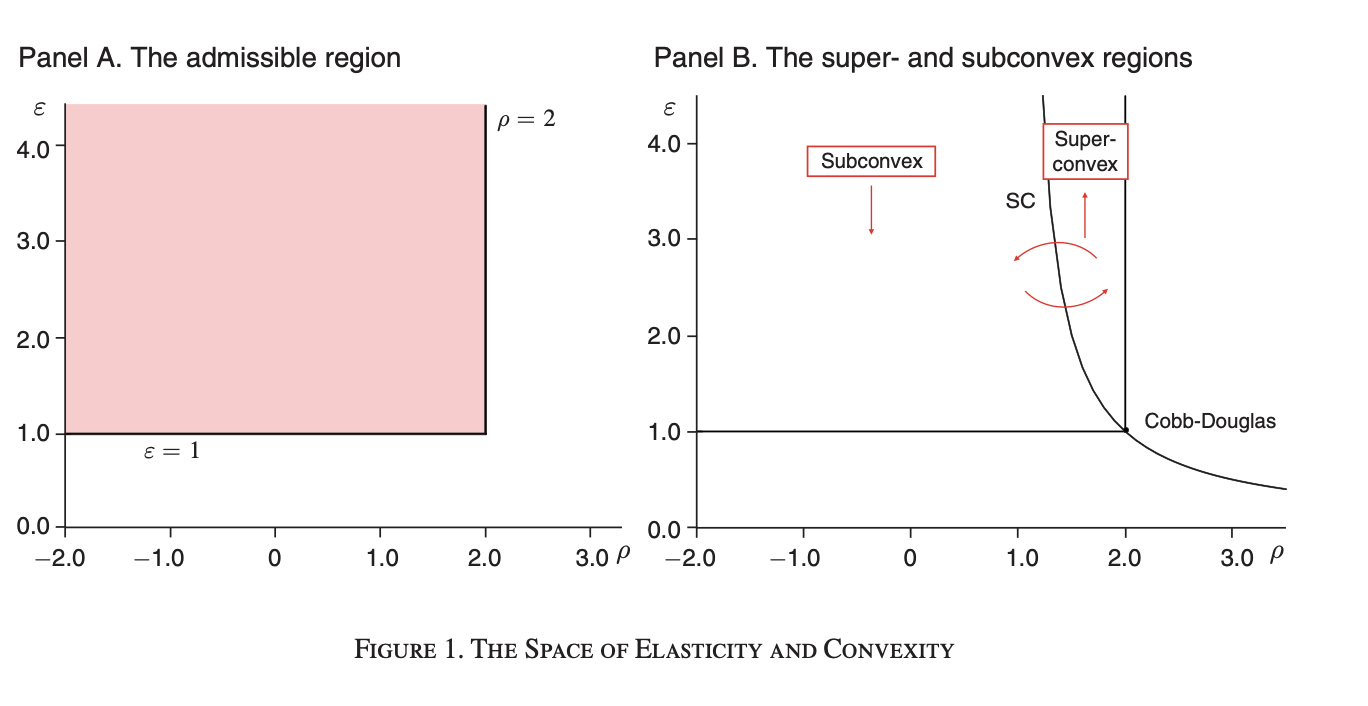
\includegraphics[width=\textwidth]{resources/neary_3}
\end{frame}


\begin{frame}{Mrázová Neary (2017)}
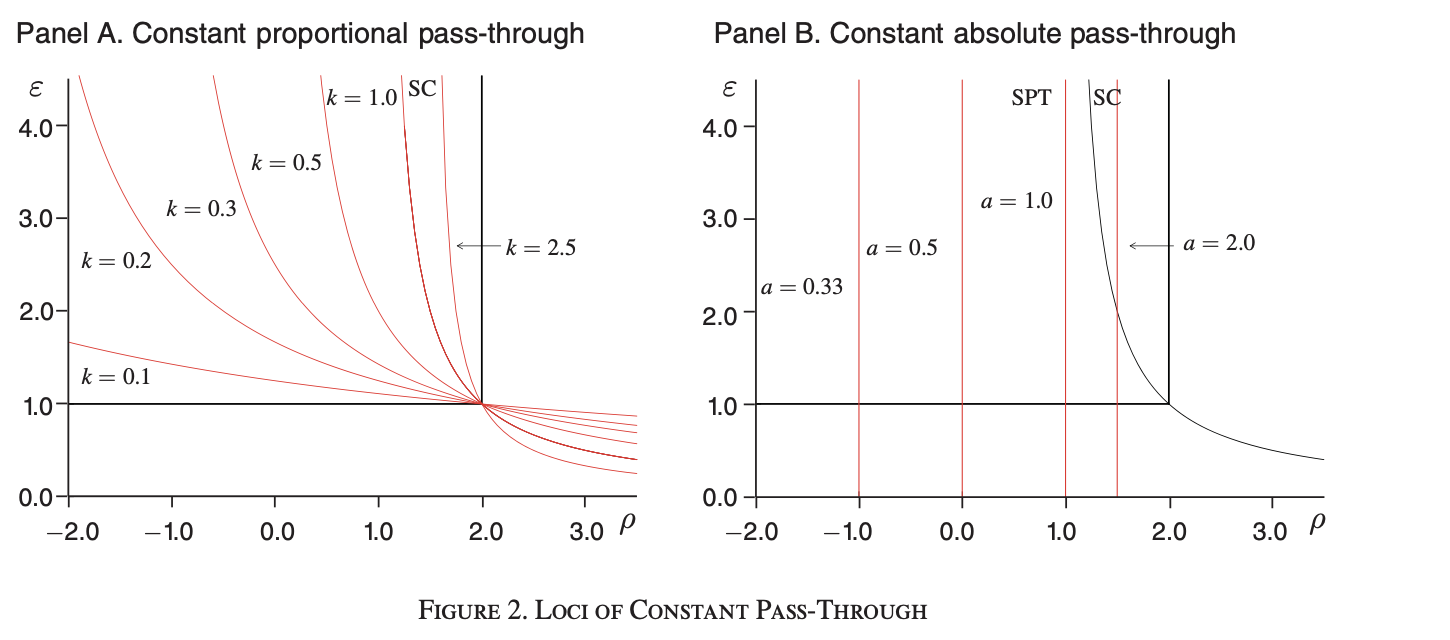
\includegraphics[width=\textwidth]{resources/neary_2}
\end{frame}



\section{Multiproduct Pass-Through}


\begin{frame}{Multiproduct Pass-Through}

\begin{itemize}
\item Most firms sell multiple products.
\item How does that affect what we know about pass-through?
\item Let's start with the case of \alert{double marginalization}.
\end{itemize}
\end{frame}

\begin{frame}{Villas Boas (ReStud 2007)/ Miller Weinberg (2017)}
Retailer and Wholesaler FOC given by:
\begin{align*}
\mathbf{p^r} &= \underbrace{\mathbf{p^w} +\mathbf{c^r}}_{\mathbf{mc^r}} -(\mathcal{H}_r \odot \Delta_{r}(\mathbf{p^r}))^{-1} \mathbf{s}(\mathbf{p^r})\\
\mathbf{p^w}  &= \mathbf{mc^w} + \left(\mathcal{H}_{w} \odot \left( \frac{\partial \mathbf{p^r}}{\partial \mathbf{p^w}} \cdot  \Delta_r(\mathbf{p^r} ) \right) \right)^{-1} \mathbf{s}(\mathbf{p^r})
\end{align*}
\begin{itemize}
  \item $\Delta_r$ is matrix of (retail) demand derivatives $\frac{\partial\, \mathbf{s}}{\partial\, \mathbf{p}}$.
\item $\mathcal{H}_r,\mathcal{H}_w$  ownership matrix $(j,k)=1$ if both products sold by same retailer/wholesaler.
\item $\frac{\partial\, \mathbf{p^r}}{\partial\, \mathbf{p^w}}$ is the \alert{pass-through matrix} (NEW!)
\end{itemize}
Challenge: We want $\mathbf{p^r}(\mathbf{p^w})$ and $\mathbf{mc^w}$ but we only have implicit solution for retailer FOC.
\end{frame}

\begin{frame}{How do we get pass-through?}
The \alert{pass-through matrix} $\frac{\partial \mathbf{p^r}}{\partial \mathbf{p^w}}$ can be obtained in one of two ways:
\begin{enumerate}
\item Numerically: perturbing the retailer's marginal costs for each possible choice of $k$ and solving
\begin{align*}
\mathbf{p^r} &=\mathbf{mc^r} + e_k -(\mathcal{H}_r \odot \Delta_{r}(\mathbf{p^r}))^{-1} \mathbf{s}(\mathbf{p^r})\\
\end{align*}
(Use Morrow Skerlos (2011) formulation and solve for every $(j,k)$ pair).
\item Analytic: Use the retailer's FOC and apply the implicit function theorem.
\begin{align}
\tag{retailer FOC}
 f(\mathbf{p^r},\mathbf{mc^r}) &\equiv \mathbf{p^r}  - \mathbf{mc^r}-  \left(\mathcal{H}_{r} \odot \Delta(\mathbf{p^r}) \right)^{-1} \mathbf{s}(\mathbf{p^r})=0 
\end{align}
See Jaffe Weyl (AEJM 2013) or Miller Weinberg (2017 Appendix E) or Conlon Rao (2023).\\
\alert{This is what PyBLP does} with \texttt{results.compute\_passthrough} (very slowly).
\end{enumerate}
\end{frame}



\begin{frame}{Multivariate IFT: Easy Part}
The multivariate IFT says that for some system of $J$ nonlinear equations 
\begin{align*}
f(\mathbf{p^r},\mathbf{p^w}) \equiv [F_1(\mathbf{p^r},\mathbf{p^w}), \ldots, F_J(\mathbf{p^r},\mathbf{p^w})]=[0,\ldots,0]
\end{align*}
with $J$ endogenous variables $\mathbf{p^r}$ and $J$ exogenous parameters $\mathbf{p^w}$.
\begin{align}
\label{eq:ptr_matrix}
\tag{PTR}
\frac{\partial \mathbf{p^r}}{\partial \mathbf{p^w}}
=-\left(\begin{array}{ccc}
\frac{\partial F_{1}}{\partial p_{1}^r} & \ldots & \frac{\partial F_{1}}{\partial p_{J}^r} \\
\ldots & \ldots & \ldots \\
\frac{\partial F_{J}}{\partial p_{1}^r} & \ldots & \frac{\partial F_{J}}{\partial p_{J}^r}
\end{array}\right)^{-1} \cdot \underbrace{\left(\begin{array}{l}
\frac{\partial F_{1}}{\partial p_{k}^w} \\
\ldots \\
\frac{\partial F_{J}}{\partial p_{k}^w}
\end{array}\right)}_{= -\mathbb{I}_J}
\end{align}
Because the system of equations is additive in $\mathbf{mc^r} = \mathbf{c^r} + \mathbf{p^w}$ this simplifies dramatically.
\end{frame}


\begin{frame}{Multivariate IFT: Hard Part}
Use the substitution $\Omega(\mathbf{p^r}) \equiv \mathcal{H}_r \odot \Delta_{r}(\mathbf{p^r})$, and differentiate the wholesalers' system of FOC's with respect to $p_l$, to get the $J \times J$ matrix with columns $l$ given by:
\begin{align}
\frac{\partial f(\mathbf{p^r},\mathbf{p^w})}{\partial p_l^r} \equiv e_l - \Omega^{-1}(\mathbf{p^r})
\left[  \mathcal{H}_{r} \odot \frac{\partial\, \Delta(\mathbf{p^r})}{\partial\, p_l^r} \right]
\Omega^{-1}(\mathbf{p^r})\,
\mathbf{s}(\mathbf{p^r}) -\Omega^{-1}(\mathbf{p^r})\, \frac{\partial \mathbf{s}(\mathbf{p^r})}{\partial p_l^r}.
\end{align}
The complicated piece is the demand Hessian: a $J \times J \times J$ tensor with elements $(j,k,l)$, $\frac{\partial^2 s_j}{\partial p_k^r \partial p_l^r} = \frac{\partial^2 \mathbf{s}}{\partial \mathbf{p^r} \partial p_l^r}=\frac{\partial\, \Delta(\mathbf{p^r})}{\partial\, p_l^r}$.\\

This also shows a key relationship between \alert{pass through} and \alert{demand curvature} (2nd derivatives).
\end{frame}



\begin{frame}{What's the point?}
Why do we care about pass-through in vertical settings?
\begin{itemize}
\item When PT is high, we think that downstream firms have siginficant market power
\item This also means the scope for \alert{elimination of double marginalization} is large.
\begin{itemize}
\item Higher pass-through should be associated with more efficient vertical mergers? (Not sure this has been tested)
\end{itemize}
\end{itemize}
\end{frame}




\begin{frame}{What's the point?}

\begin{itemize}
\item Because second-derivatives of plain logit are pinned down by price coefficient and shares, we don't have any flexibility in curvature.
\item Mixed logit is less restricted but how much less? (See Miravete Seim Thurk 2023 at CEPR)
\item Probably these models are under-parametrized....but
\item A huge class of models adds an extra parameter between wholesale and retail prices...2
\end{itemize}
\end{frame}



\section{Estimating Pass Through: Conlon Rao (AEJP: 2020)}

\begin{frame}{A simple empirical exercise}
\begin{itemize}
\item US states tax distilled spirits by volume
\item We see tax changes in three states (Connecticut, Louisianna, Illinois)
\item Three popular bottle sizes (750mL, 1L, 1.75L)
\item Run a regression at a 3 month difference product by product
\begin{align*}
\Delta p_{j s t}=\rho_{j s t}(\mathbf{X}, \Delta \tau) \cdot \Delta \tau_{j t}+\beta \Delta x_{j s t}+\gamma_j+\gamma_t+\epsilon_{j s t}
\end{align*}
\item Only innovation: allow $\rho_{j s t}(\mathbf{X}, \Delta \tau) $ to vary by size of tax increase.
\end{itemize}
\end{frame}


\begin{frame}{Goes horribly wrong}
\begin{columns}
\begin{column}{0.4\textwidth}
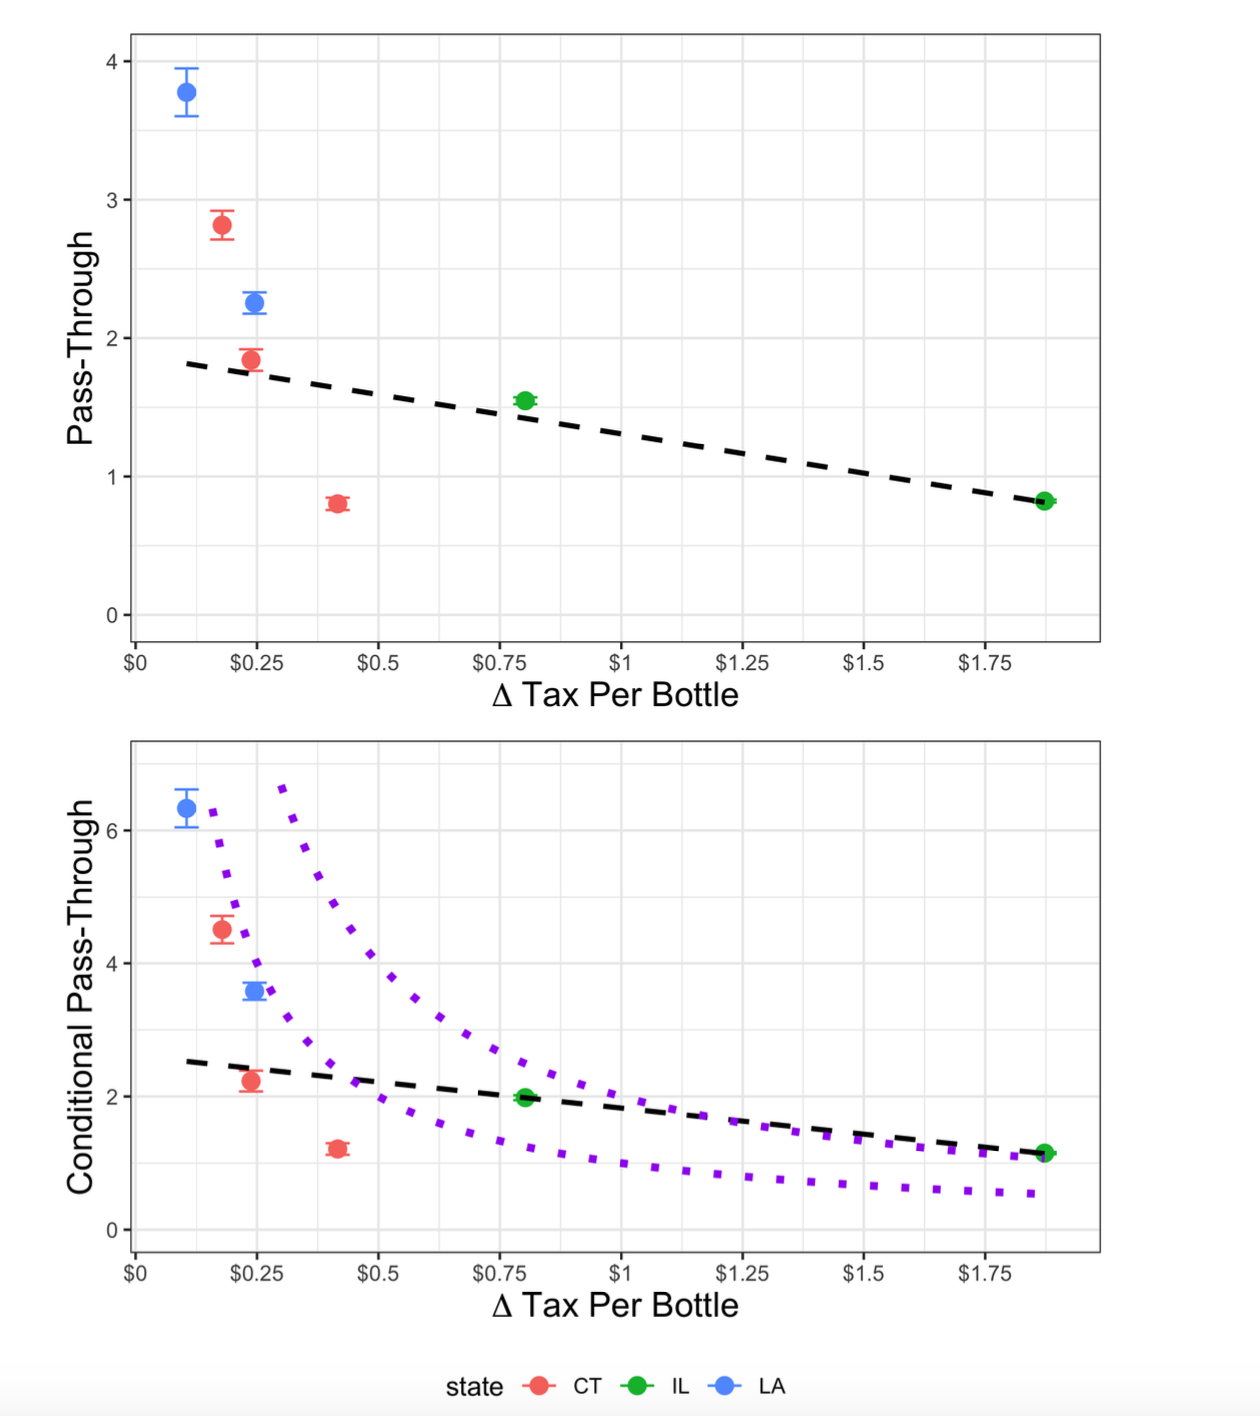
\includegraphics[height=0.9\textheight]{resources/cr_1.png}
\end{column}
\begin{column}{0.5\textwidth}
\begin{itemize}
\item Regression coefficients are huge $>1$ and all over the map
\item Conditional on a price change even larger $>3$
\item Seem to coincide with the purple line 
\end{itemize}
\end{column}
\end{columns}
\end{frame}


\begin{frame}{Is PT a structural parameter?}
\begin{columns}
\begin{column}{0.5\textwidth}
\begin{itemize}
\item Price points are a big problem here
\item Estimated an ordered probit with flexible $\beta(\Delta \tau)$
\item Pass-through depends on where you are; not stable at all (!)
\item Maybe structural interpretations of pass-through parameter are a bad idea!
\end{itemize}
\end{column}
\begin{column}{0.5\textwidth}
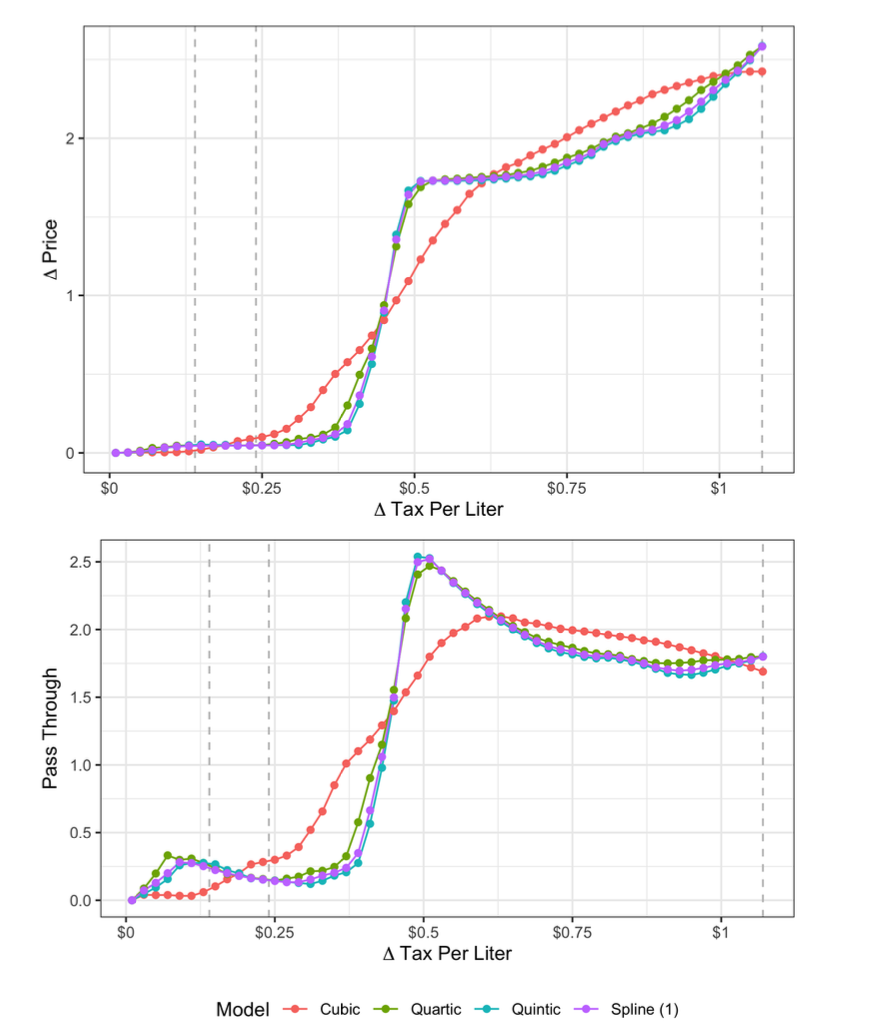
\includegraphics[height=0.9\textheight]{resources/cr_3.png}
\end{column}
\end{columns}
\end{frame}

\begin{frame}{Some challenges}
\begin{itemize}
\item Pless and Van Bentham (AEJA: 2019)\\
 Use pass-through $>1$ as a test for market power? (Is this true?)
\item Chetty Looney Croft (AER 2016)
\begin{align*}
\log q\left(p, \tau^S\right)&=\alpha+\beta \log p+\theta_\tau \beta \log \left(1+\tau^S\right)\\
\theta_\tau&=\frac{\partial \log q}{\partial \log \left(1+\tau^S\right)} / \frac{\partial \log q}{\partial \log p}=\frac{\varepsilon_{q, 1+\tau^s}}{\varepsilon_{q, p}}
\end{align*}
\item Use $\theta$ as evidence of ``tax salience'' (is it?)
\item Can we identify markups... ?!?
\end{itemize}
\end{frame}




% \begin{frame}{Pass-through Counterfactuals? (Conlon Rao 2023)}
% \footnotesize
% How do we solve for $p^w$ under a counterfactual pass-through matrix?
% \begin{itemize}
% \item Idea: pass-through only augments the matrix $\Delta_r(\mathbf{p^r})$.
% \item Example: a constant sales tax rate $P \equiv \frac{\partial \mathbf{p^r}}{\partial \mathbf{p^w}} = \text{diag}(1+\tau_r)$
% \end{itemize}
% \begin{align*}
% \mathbf{p^w}  &= \mathbf{mc^w} + \left(\mathcal{H}_{w} \odot \left( \frac{\partial \mathbf{p^r}}{\partial \mathbf{p^w}} \cdot  \Delta_r(\mathbf{p^r} ) \right) \right)^{-1} \mathbf{s}(\mathbf{p^r})
% \end{align*}
% Adapt the Morrow Skerlos $\zeta$ fixed point where $P \Delta(\boldsymbol{p}_t) = P \Lambda_t\left(\boldsymbol{p}_t\right)- P \Gamma_t\left(\boldsymbol{p}_t\right)$
% \begin{align*}
% \boldsymbol{p}_t &\leftrightarrow \boldsymbol{c}_t+\boldsymbol{\zeta}_t\left(\boldsymbol{p}_t\right) \quad \text { where }\\
%  \boldsymbol{\zeta}_t\left(\boldsymbol{p}_t\right)&=\Lambda_t\left(\boldsymbol{p}_t\right)^{-1} \alert{P^{-1}}\left[\mathcal{H}_t^* \odot \alert{P}\, \Gamma_t\left(\boldsymbol{p}_t\right)\right]\left(\boldsymbol{p}_t-\boldsymbol{c}_t\right)-\Lambda_t\left(\boldsymbol{p}_t\right)^{-1} \alert{P^{-1}} \boldsymbol{s}_t\left(\boldsymbol{p}_t\right)
% \end{align*}
% For diagonal $P$ (not sure about general case with Hadamard product):
% \begin{align*}
%  \boldsymbol{\zeta}_t\left(\boldsymbol{p}_t\right)=\Lambda_t\left(\boldsymbol{p}_t\right)^{-1}\left[\mathcal{H}_t^* \odot  \Gamma_t\left(\boldsymbol{p}_t\right)\right]\left(\boldsymbol{p}_t-\boldsymbol{c}_t\right)-\Lambda_t\left(\boldsymbol{p}_t\right)^{-1} \alert{P^{-1}} \boldsymbol{s}_t\left(\boldsymbol{p}_t\right)
% \end{align*}
% \end{frame}








% \begin{columns}
% \begin{column}{0.5\textwidth}
% 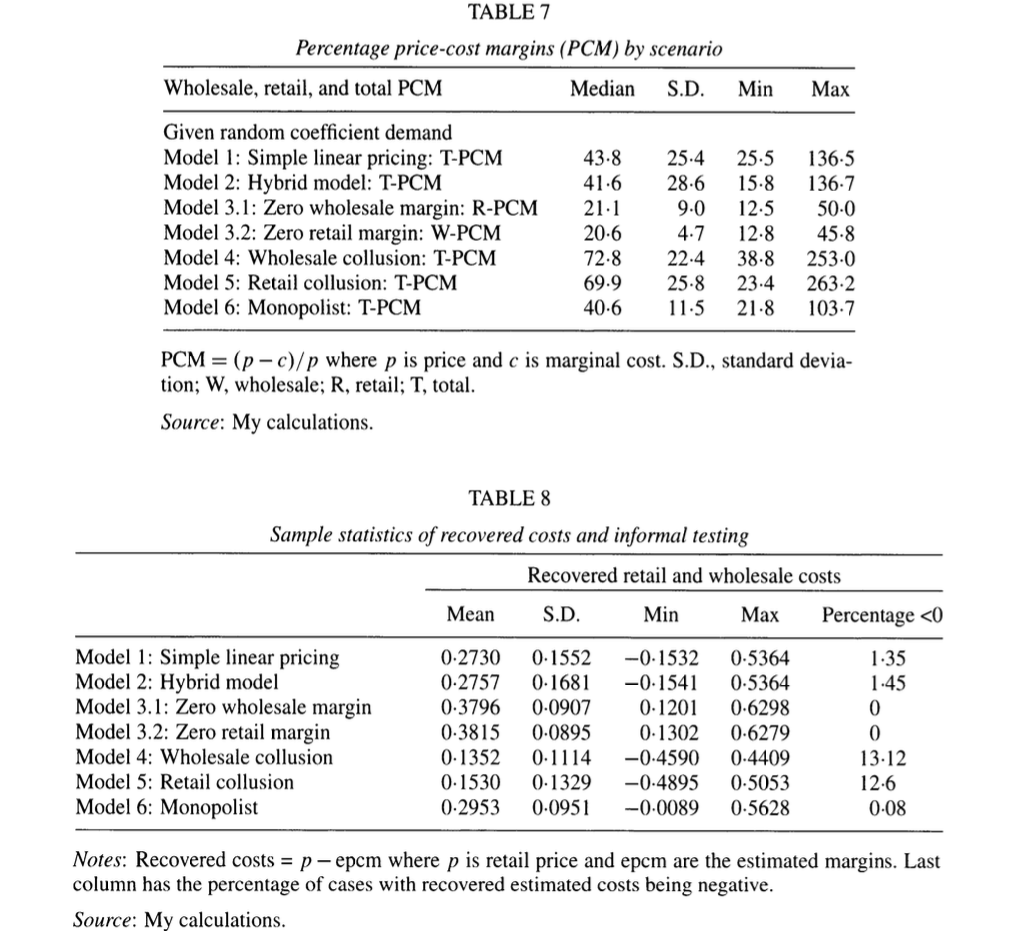
\includegraphics[height=0.9\textheight]{resources/villas_boas_table8.png}
% \end{column}
% \begin{column}{0.5\textwidth}
% \begin{itemize}
% \item Try out different models of price setting behavior, compute $\eta$ markups.
% \item Unsurprisingly models with higher markups also have more costs $MC < 0$.
% \item Is this evidence of incorrect conduct assumption or inelastic demand?
% \end{itemize}
% \end{column}
% \end{columns}
% \end{frame}






\end{document}

